\section{Motivation}

In this section, we motivate the need for declarative reasoning for eventually
consistent data store.

\subsection{System Model}

We assume a system model where the eventually consistent database is organized
as a collection of key-indexed, object-valued tables. The objects stored in the
tables are instances of the same replicated data type. The database is composed
of a number of \emph{replicas}, and each object is fully replicated across all
the replicas. Under this model, a client request for an operation with no
application-level consistency requirement can be serviced if at least one of
the replicas is reachable. Thus, with the addition of new replicas, and placing
them close to the clients, leads to improved throughput and reduced latencies.

\subsection{Bank account database}

Suppose our goal is to implement a bank account service on top an eventually
consistent data store, with the following schema,

\begin{codesql}
Create Table BankAccount (
  userID int PRIMARY KEY,
  userName string UNIQUE,
  balance float CHECK (balance >= 0))
\end{codesql}

\noindent with the following \emph{operations}.

\begin{codehaskell}
type UserName = String
-- returns false if the user name is already taken
addAccount     :: UserName -> Bool
getBalanceName :: UserName -> Float
depositName    :: UserName -> Float -> ()
-- returns false if the account has insufficient balance
withdrawName   :: UserName -> Float -> Bool
\end{codehaskell}

Notice that the operations manipulating the table take user name as input.
Since eventually consistent databases are non-relational~\cite{}, we need to
maintain a \emph{secondary index} to look up records by user name.

\begin{codesql}
Create Table UserIndex (
  userName string PRIMARY KEY,
  userID int
  FOREIGN KEY (userID)
    REFERENCES BankAccount (userID) )
\end{codesql}

\begin{figure}[t]
\centering
\subfigure[Negative Balance]{\label{fig:negativeBalanceAnomaly}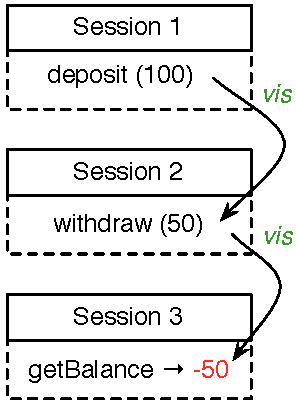
\includegraphics[width=0.31\columnwidth]{Figures/Motivation2}}
\hfill
\subfigure[Missing update]{\label{fig:missingUpdateAnomaly}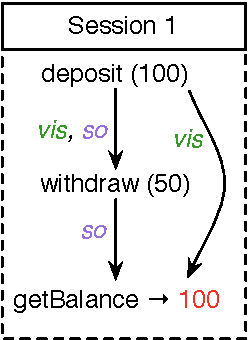
\includegraphics[width=0.26\columnwidth]{Figures/Motivation1}}
\hfill
\subfigure[Monotonicity violation]{\label{fig:monotonicityAnomaly}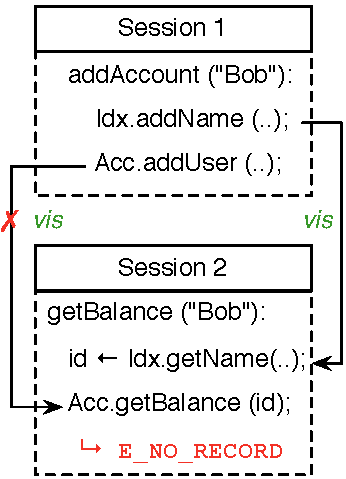
\includegraphics[width=0.36\columnwidth]{Figures/Motivation3}}
\caption{Anomalies possible under eventual consistency for the get balance operation.}
\label{fig:cleanliness_examples}
\end{figure}

\subsection{Anomalies}

In a traditional database system, the programmer need only to define the
application-level integrity constraints along with the schema, and the database
management system automatically enforces the necessary coordination. However,
under eventual consistency, the onus is on the programmer to ensure not only
that the integrity constraints are preserved, but also to prevent any
inconsistencies being exposed to the user. For example, it is easy to see that
the withdraw operations must be strongly consistent operations to preserve the
integrity constraint. However, it is possible that the get balance operation
still returns a negative balance.

Figure~\ref{fig:negativeBalanceAnomaly} illustrates such a potential execution.
Assume that all operations are on the same object, and the balance on the
account was initially 0. Here, \cf{vis} edges capture the visibility
relation between the operations. In this case, the withdraw sees the deposit,
but the get balance operation only witnesses the withdraw. Such an execution is
possible under eventual consistency, where the \emph{effect} (update)
corresponding to the withdraw reaches the replica to which the get balance is
applied to before the causally preceding deposit effect. Alternatively, it is
possible that a get balance operation does not see the effects from its own
session (Figure~\ref{fig:missingUpdateAnomaly}), leading the user to
incorrectly conclude that the previous update failed to go through. Here, the
\cf{so} edge represents the session order that exists between the actions
on the same thread.

The anomalies discussed so far arise from weakly consistent behaviors on the
same object. With operations on multiple objects on distinct tables, the
programmer on eventually consistent databases has to take care of preserving
integrity constraints for foreign keys, materialized views and secondary
indexes. For example, Figure~\ref{fig:monotonicityAnomaly} illustrates the
anomaly that arises from the lack of monotonic update visibility. Adding a new
account involves a conditional insertion into the index table, followed by an
insertion into the bank account table. Many eventually consistent data stores
propose write-only transactions~\cite{}, and let us assume that add user
operation is marked as a write-only transaction. Despite this, under eventual
consistency, it is possible for a \cf{getBalanceName} operation to witness the
first insertion but not the second, exposing an inconsistent state. The two
reads may be served by different replicas, where the only the former has
witnessed the effects of add user transaction. Assigning the correct store
consistency level for the operations in this example such that the
application-level constraints are preserved is a non-trivial task.

\subsection{Implementation in Quelea}

Quelea automates this error-prone task; the programmer need only to express the
application-level consistency constraints in the contract language. Replicated
data types in Quelea are defined as reductions over the set of effects similar
to operation-based CRDTs~\cite{}. The following data type definitions capture
the operations and effects on the bank account and user index objects.

\begin{codehaskell}
data BankAcc = AddUser UserName | Deposit Float
             | Withdraw Float | GetBalance
data UserIdx = AddName UserID | GetName
\end{codehaskell}

Recall that the key of the bank account table is user id, which maps to a
particular bank account object. In Quelea, an object state is nothing but the
set of effects (called the \emph{context}) on this object. As such,
\cf{Deposit} and \cf{Withdraw} effects simply include the amount deposited or
withdrawn, and \cf{AddUser} effect includes the user name. Similarly, on the
user index table, where the key is user name, the value is simply an effect
(\cf{AddName}) binding some user id at this key. \cf{GetBalance} and
\cf{GetName} correspond to the corresponding read-only operations. The complete
definition of the operations on bank account and user index objects is given
below.

\begin{codehaskell}
-- Get balance takes no arguments and read-only
getBalance :: [BankAcc] {- context -} -> () {- args -}
  -> (() {- ret val -}, Maybe BankAcc {- effect -})
getBalance ctxt _ = (sum [v | Deposit v (- ctxt]
        - sum [v | Withdraw v (- ctxt], Nothing)

-- withdraw returns True on success
withdraw :: [BankAcc] -> Float -> (Bool, Maybe BankAcc)
withdraw c v = if sel1 $ getBalance c () >= v
               then (True, Just $ Withdraw v)
               else (False, Nothing)

deposit :: [BankAcc] -> v -> ((), Maybe BankAcc)
deposit _ v = ((), Just $ Deposit v)

addUser :: [BankAcc] -> UserName -> ((), Maybe BankAcc)
addUser _ n = ((), Just $ AddUser n)

addName :: [UserIdx] -> UserID -> (Bool, Maybe UserIdx)
addName [] uid = (True, Just $ AddName uid)
addName x:_ _ = (False, Nothing)

getName :: [UserIdx] -> ()
        -> (Maybe UserName, Maybe UserIdx)
getName [] _ = (Nothing, Nothing)
getName (AddUser uid:_) _ = (Just uid, Nothing)
\end{codehaskell}

The definitions are a straight forward encoding of the expected behavior.
Quelea programming model provides the programmer complete freedom regarding the
semantics and desired convergence property of the replicated data type, and
indeed, we can encode the well-known CRDTs~\cite{SSS} in a declarative fashion.
Observe that the operation definitions presented here only capture the
convergence properties of the replicated data type, and are not concerned with
the consistency properties, which is expressed through the contract language.

\subsection{Contracts}

The contract for the strongly consistent \cf{addName} operation is given below:
\begin{smathpar}
\begin{array}{l}
\rsf{addNameCtrt} = \forall (a:\rsf{AddName}). \\
\qquad \sameobj{a}{\cureff} \Rightarrow \vis{a}{\cureff} \vee \vis{\cureff}{a} \vee a = \cureff
\end{array}
\end{smathpar}

In the above definition, $\cureff$ represents the current effect --- the effect
emitted by the \cf{addName} operation. The contract simply states our
high-level observation; for any effect $a$ which is also an \cf{AddName} effect
on the same object, it must be the case that $a$ is visible to $\cureff$ or
vice verse, or $a$ is $\cureff$. Here, $\sameobjZ$ and $\visZ$ are primitive
relations. This contract ensures that any two \cf{addName} operations will be
seen by each other. The contract for withdraw is similar to the
\cf{addNameCtrt}.

Since the deposit operation does not have any restrictions, its contract is
simply $\true$. Same is the case for \cf{addUser} operation. The contract for
get balance operation is:
\begin{smathpar}
\begin{array}{l}
\rsf{getBalCtrt} = \forall (a:\rsf{Deposit}), (b:\rsf{Withdraw}). \\
\qquad \vis{a}{b} \wedge \vis{b}{\cureff} \Rightarrow \vis{a}{\cureff} \\
\qquad \vee (\soZ \cap \sameobjZ) (a,\cureff) \Rightarrow \vis{a}{\cureff} \\
\qquad \vee (\soZ \cap \sameobjZ) (b,\cureff) \Rightarrow \vis{b}{\cureff}
\end{array}
\end{smathpar}

If a withdraw $b$ is visible to the get balance operation, then all deposit
operations $a$ visible to withdraw should be visible to the get balance
operation. This prevents negative balance anomalies. The rest of the contract
says that a get balance operation must witness previous deposit and withdraw
operations on the same object in the same session. This prevents missed update
anomalies.

Similar to contracts on operations, Quelea supports contracts on transactions.
The contract on the \cf{getBalanceName} transaction is given below:
\begin{smathpar}
\begin{array}{l}
\rsf{getBalanceNameCtrt} = \forall (a:\rsf{GetName}), (b:\rsf{GetBalance}), \\
\quad (c:\rsf{AddName}), (d:\rsf{AddUser}). ~\trans{a}{b}{c}{d} \wedge \so{a}{b} \\
\qquad \wedge ~\vis{c}{a} \wedge \sameobj{d}{b} \Rightarrow \vis{d}{b}
\end{array}
\end{smathpar}

$\trans{a}{b}{c}{d}$ says that the action pairs $a,b$ and $c,d$ are in the same
transaction, and the two transactions are distinct. The contract says
specifically forbids the anomaly presented in
Figure~\ref{fig:monotonicityAnomaly}. This is the desired semantics for the
\cf{getUserName} transaction.

The programmer simply defines such contracts on the operations and the
transactions. Quelea logically analyzes the contracts, and maps the
corresponding operation to the precise store consistency and isolation level.
Thus, Quelea equips the programmer with a declarative model for reasoning and
expressing eventually consistent programs.
